\section{Simulating the LOB}
\subsection{Example Code}
We present code written that is relevant for this thesis to demonstrate use of the Coinbase Pro API. Development was done in Python using a Jupyter notebook. We use of CoPrA, an asynchronous web socket client for Coinbase Pro (\cite{L3}), to obtain LOB data with real time updates. The Coinbase Pro API provides us with a snapshot of LOB data that includes the price and volume of every bid and ask for an asset (consolidated so that orders of the same price are combined). By opening up a web socket, we also receive updates of all trades at each position of the LOB. The following code shows preliminary work using the API to model the dynamics of the “ETC-USD” orderbook, which is the exchange of Ethereum Classic for USD (around \$2 million volume of trades each day). We start with the snapshot of the LOB to create our own internal representation of the LOB. We then update the order book whenever we receive an event from the API (which consists of a timestamp, price, and new volume). We update the order book with every event, and also calculate the $AES$ for the first 5 bids and asks ($K=5$ in the queue reactive model from above). Although the LOB further extends on both sides, we assume that the majority of trades occur in the first $K$ bids and asks. The code could also be adapted to estimate $\lambda_i(q)$, and $\gamma_i(q)$ for each $i$ by using the time stamps of the events. The code is displayed in Listing ~\ref{AESCode}:

\lstinputlisting[language=Python, caption=Receiving LOB Data from Coinbase Pro and Calculating AES, label=AESCode]{Code/AES}

Sample output is shown in Figure \ref{fig:LOB_pic} and Listing \ref{AESOutput1}. This includes the plot of the LOB from when we take the first snapshot as well as the first update.

\begin{figure}[t]
\begin{center}
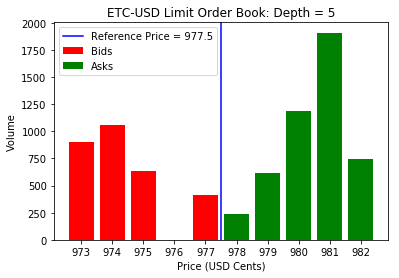
\includegraphics[width=0.8\textwidth]{Figures/LOB_Picture.png}
\caption{LOB Sample}
\label{fig:LOB_pic}
\end{center}
\end{figure}

\lstinputlisting[language={}, caption=Processing Next Order and Updating LOB, label=AESOutput1]{Code/first_update}

After 3 minutes, we have the following order book and $AES$’s (Listing \ref{AESOutput2}) 

\lstinputlisting[language={}, caption=Updated LOB after 3 Minutes, label=AESOutput2]{Code/later_update}

As can be seen, the reference price went from \$9.775 to \$9.745, possibly due to large taker order from the ask side. For the actual thesis work, we would run the code for a much longer (possibly multiple days) time to estimate $AES$, $\lambda_(q)$, and $\gamma_i(q)$ for each $i$.

\subsection{Using Parameters to Simulate LOB}
Here, I will use the values that I estimated from above to write a program that simulates the LOB using the queue reactive model.

\section{Reinforcement Learning Model}
\subsection{Reinforcement Learning Background}
Here, I will provide background on reinforcement learning that is necessary to understand the experiment and why it is a good choice for this problem.
\subsection{Machine Learning Architecture}
Here, I will describe the programming environment and machine learning model for the problem.